\documentclass{standalone}
\usepackage{tikz}

\begin{document}
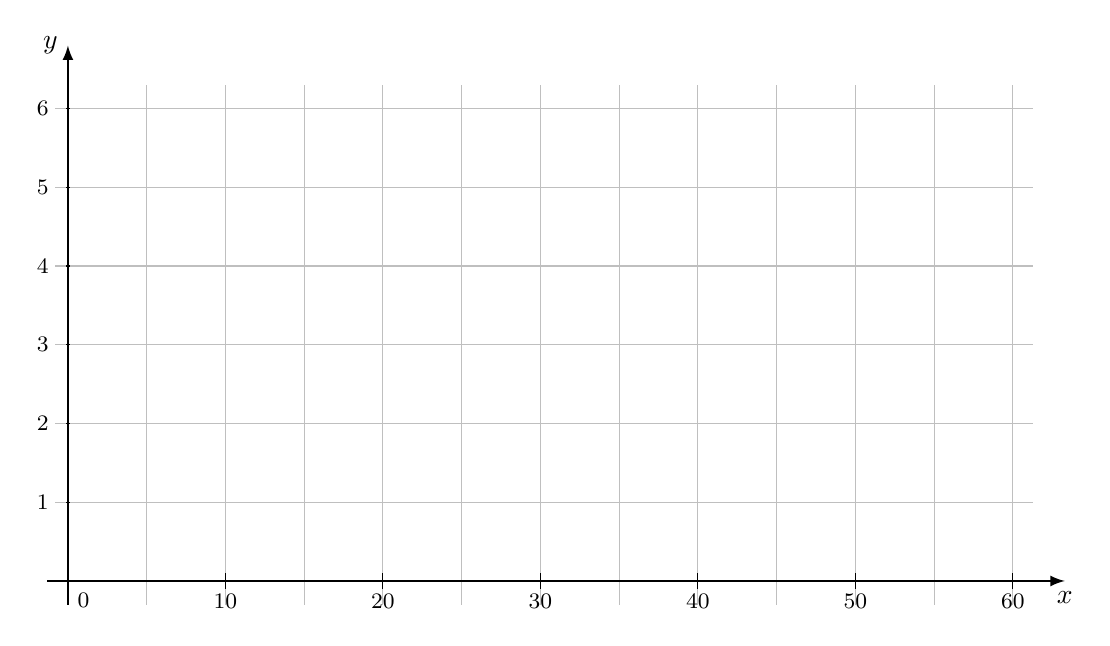
\begin{tikzpicture}[cross/.style={draw, cross out, minimum size=2*(#1-1pt), inner sep=0pt, outer sep=0pt}, x=2mm, y=10mm,
    >=latex,   %Voreinstellung für Pfeilspitzen
    font= \footnotesize, scale=1]
    %Raster zeichnen
    \draw [color=gray!50]  [step=10mm] (-0.8,-0.3) grid (61.3,6.3);
    % Achsen zeichnen
    \draw[->,thick] (-1.3,0) -- (63.3,0) node[right, below] {\normalsize $x$};
    \draw[->,thick] (0,-0.3) -- (0,6.8) node[above, left] {\normalsize $y$};
    % Achsen beschriften
    \foreach \x in {10,20,...,60} \draw (\x,-.1) -- (\x,.1) node[below=4pt] {$\x$};
    \foreach \y in {1,2,...,6} \draw (-.1,\y) -- (.1,\y) node[left=4pt] {$\y$};
    % Besserer Ursprung
    \draw[color=black] (0pt,-7pt) node[right] {$0$};
    %Funktionen zeichnen:
    \clip(-0.3,-0.3) rectangle (60.8,6.8); %Bildbereich
    %Beschriftung
    %\node[blue]  at (11,5) {\normalsize$f$};
\end{tikzpicture}


\end{document}